\tikzset{
    arg/.style={
        draw,
        circle,
        fill=gray!15,
        inner sep=1pt,
        minimum size=.5cm
    },
    auxiliary/.style={
        arg,
        fill=gray!30
    },
    attack/.style={
        ->,
        thick,
        >=stealth
    }
}

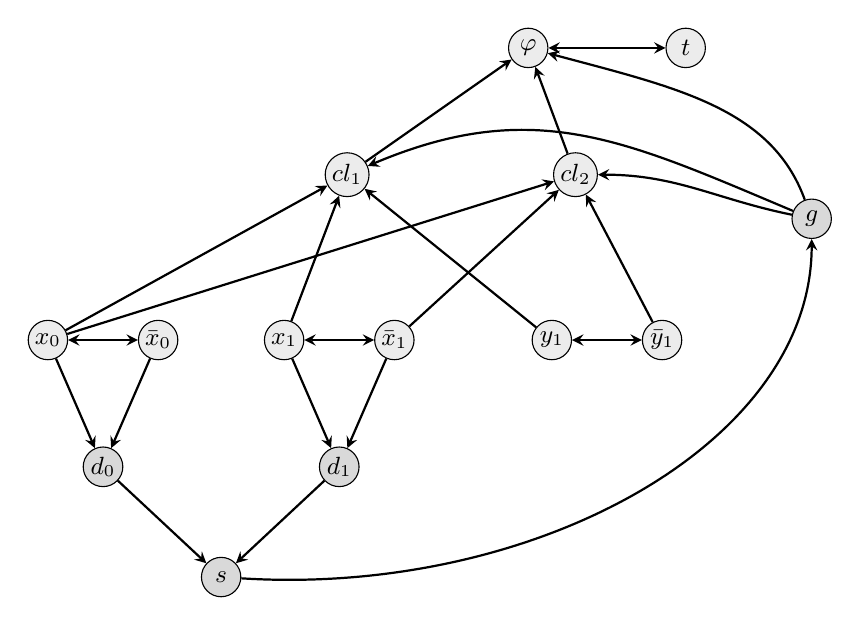
\begin{tikzpicture}[>=stealth,xscale=1, yscale=0.7]
\small

    % Formel-, Klausel- und Hilfsargumente
    \path
        node[arg]       at ( 1.2,  .3) (phi) {$\varphi$}
        node[arg]       at ( 3.2,  .3) (t)   {$t$}
        node[arg]       at (-1.1,-2.0) (cl1)  {$cl_1$}
        node[arg]       at ( 1.8,-2.0) (cl2)  {$cl_2$}
        node[auxiliary] at ( 4.8,-2.8) (g)   {$g$};

    % Literalargumente
    \path
        node[arg] at (-4.9,-5.0) (x0)  {$x_0$}
        node[arg] at (-3.5,-5.0) (nx0) {$\bar{x}_0$}
        node[arg] at (-1.9,-5.0) (x1)  {$x_1$}
        node[arg] at (-0.5,-5.0) (nx1) {$\bar{x}_1$}
        node[arg] at ( 1.5,-5.0) (y1)  {$y_1$}
        node[arg] at ( 2.9,-5.0) (ny1) {$\bar{y}_1$};

    % Unteres Hilfsgadget
    \path
        node[auxiliary] at (-4.2,-7.3) (d0) {$d_0$}
        node[auxiliary] at (-1.2,-7.3) (d1) {$d_1$}
        node[auxiliary] at (-2.7,-9.3) (s)  {$s$};

    % Symmetrische Angriffe werden durch eine Kante mit zwei
    % Pfeilspitzen dargestellt.
    \path[attack,<->]
        (x0)  edge (nx0)
        (x1)  edge (nx1)
        (y1)  edge (ny1)
        (phi) edge (t);

    % Literale greifen die Klauseln an, in denen sie vorkommen
    \path[attack]
        (x0)  edge (cl1)
              edge (cl2)
        (x1)  edge (cl1)
        (y1)  edge (cl1)
        (nx1) edge (cl2)
        (ny1) edge (cl2);

    % Klauselargumente greifen das Formelargument an
    \path[attack]
        (cl1) edge (phi)
        (cl2) edge (phi);

    % d- und s-Gadget
    \path[attack]
        (x0)  edge (d0)
        (nx0) edge (d0)
        (x1)  edge (d1)
        (nx1) edge (d1)
        (d0)  edge (s)
        (d1)  edge (s)
        (s)   edge[out=-5,in=-90,looseness=1] (g);

    % Angriffe des g-Arguments
    \path[attack]
        (g) edge[out=150,in=30,looseness=1.15] (cl1)
            edge[out=165,in=0] (cl2)
            edge[out=105,in=-20,looseness=1.05] (phi);
\end{tikzpicture}
